\subsubsection{Overview}
The Breath First Search (BFS) is another fundamental search algorithm used to explore nodes and edges of a graph. It runs with a time complexity of $O(V + E)$ and is often used as a building block in other algorithms.

The BFS algorithm is particularly useful for one thing: finding the shortest path on unweighted graphs. Let's show the next graph.

\begin{figure}[H]
\begin{center}
    \begin{tikzpicture}[scale=0.2]
    \tikzstyle{every node}+=[inner sep=0pt]
    \draw [black] (35.4,-45.9) circle (3);
    \draw (35.4,-45.9) node {$0$};
    \draw [black] (35.4,-45.9) circle (2.4);
    \draw [black] (18.6,-38.7) circle (3);
    \draw (18.6,-38.7) node {$9$};
    \draw [black] (51.5,-54.2) circle (3);
    \draw (51.5,-54.2) node {$11$};
    \draw [black] (4.6,-31.2) circle (3);
    \draw (4.6,-31.2) node {$10$};
    \draw [black] (18.6,-25) circle (3);
    \draw (18.6,-25) node {$1$};
    \draw [black] (31.1,-31.2) circle (3);
    \draw (31.1,-31.2) node {$8$};
    \draw [black] (48.1,-38.7) circle (3);
    \draw (48.1,-38.7) node {$7$};
    \draw [black] (66.4,-36.7) circle (3);
    \draw (66.4,-36.7) node {$6$};
    \draw [black] (45.9,-24.2) circle (3);
    \draw (45.9,-24.2) node {$3$};
    \draw [black] (53.6,-10.8) circle (3);
    \draw (53.6,-10.8) node {$4$};
    \draw [black] (72.9,-23.3) circle (3);
    \draw (72.9,-23.3) node {$5$};
    \draw [black] (39.1,-8.3) circle (3);
    \draw (39.1,-8.3) node {$2$};
    \draw [black] (26.9,-14.4) circle (3);
    \draw (26.9,-14.4) node {$12$};
    \draw [black] (32.64,-44.72) -- (21.36,-39.88);
    \draw [black] (38.07,-47.27) -- (48.83,-52.83);
    \draw [black] (38.01,-44.42) -- (45.49,-40.18);
    \draw [black] (48.74,-41.63) -- (50.86,-51.27);
    \draw [black] (21.17,-37.16) -- (28.53,-32.74);
    \draw [black] (15.96,-37.28) -- (7.24,-32.62);
    \draw [black] (7.34,-29.99) -- (15.86,-26.21);
    \draw [black] (28.41,-29.87) -- (21.29,-26.33);
    \draw [black] (51.08,-38.37) -- (63.42,-37.03);
    \draw [black] (47.65,-35.73) -- (46.35,-27.17);
    \draw [black] (47.39,-21.6) -- (52.11,-13.4);
    \draw [black] (67.71,-34) -- (71.59,-26);
    \draw [black] (44.72,-21.44) -- (40.28,-11.06);
    \draw [black] (30.37,-28.29) -- (27.63,-17.31);
    \draw [black] (29.58,-13.06) -- (36.42,-9.64);
    \end{tikzpicture}
    \end{center}
\end{figure}

If we start in the node 0, using the BFS then we need to move to the neighborhoods of the current node, so we get the next:

\begin{figure}[H]
\begin{center}
    \begin{tikzpicture}[scale=0.2]
    \tikzstyle{every node}+=[inner sep=0pt]
    \draw [black] (35.4,-45.9) circle (3);
    \draw (35.4,-45.9) node {$0$};
    \draw [black] (35.4,-45.9) circle (2.4);
    \draw [black] (18.6,-38.7) circle (3);
    \draw (18.6,-38.7) node {$9$};
    \draw [black] (18.6,-38.7) circle (2.4);
    \draw [black] (51.5,-54.2) circle (3);
    \draw (51.5,-54.2) node {$11$};
    \draw [black] (51.5,-54.2) circle (2.4);
    \draw [black] (4.6,-31.2) circle (3);
    \draw (4.6,-31.2) node {$10$};
    \draw [black] (18.6,-25) circle (3);
    \draw (18.6,-25) node {$1$};
    \draw [black] (31.1,-31.2) circle (3);
    \draw (31.1,-31.2) node {$8$};
    \draw [black] (48.1,-38.7) circle (3);
    \draw (48.1,-38.7) node {$7$};
    \draw [black] (48.1,-38.7) circle (2.4);
    \draw [black] (66.4,-36.7) circle (3);
    \draw (66.4,-36.7) node {$6$};
    \draw [black] (45.9,-24.2) circle (3);
    \draw (45.9,-24.2) node {$3$};
    \draw [black] (53.6,-10.8) circle (3);
    \draw (53.6,-10.8) node {$4$};
    \draw [black] (72.9,-23.3) circle (3);
    \draw (72.9,-23.3) node {$5$};
    \draw [black] (39.1,-8.3) circle (3);
    \draw (39.1,-8.3) node {$2$};
    \draw [black] (26.9,-14.4) circle (3);
    \draw (26.9,-14.4) node {$12$};
    \draw [black] (32.64,-44.72) -- (21.36,-39.88);
    \draw [black] (38.07,-47.27) -- (48.83,-52.83);
    \draw [black] (38.01,-44.42) -- (45.49,-40.18);
    \draw [black] (48.74,-41.63) -- (50.86,-51.27);
    \draw [black] (21.17,-37.16) -- (28.53,-32.74);
    \draw [black] (15.96,-37.28) -- (7.24,-32.62);
    \draw [black] (7.34,-29.99) -- (15.86,-26.21);
    \draw [black] (28.41,-29.87) -- (21.29,-26.33);
    \draw [black] (51.08,-38.37) -- (63.42,-37.03);
    \draw [black] (47.65,-35.73) -- (46.35,-27.17);
    \draw [black] (47.39,-21.6) -- (52.11,-13.4);
    \draw [black] (67.71,-34) -- (71.59,-26);
    \draw [black] (44.72,-21.44) -- (40.28,-11.06);
    \draw [black] (30.37,-28.29) -- (27.63,-17.31);
    \draw [black] (29.58,-13.06) -- (36.42,-9.64);
    \end{tikzpicture}
\end{center}
\end{figure}

Again we choose arbitrarily a new node for example the node 9 and we repeat the same process.

\begin{figure}[H]
\begin{center}
    \begin{tikzpicture}[scale=0.2]
    \tikzstyle{every node}+=[inner sep=0pt]
    \draw [black] (35.4,-45.9) circle (3);
    \draw (35.4,-45.9) node {$0$};
    \draw [black] (35.4,-45.9) circle (2.4);
    \draw [black] (18.6,-38.7) circle (3);
    \draw (18.6,-38.7) node {$9$};
    \draw [black] (18.6,-38.7) circle (2.4);
    \draw [black] (51.5,-54.2) circle (3);
    \draw (51.5,-54.2) node {$11$};
    \draw [black] (51.5,-54.2) circle (2.4);
    \draw [black] (4.6,-31.2) circle (3);
    \draw (4.6,-31.2) node {$10$};
    \draw [black] (4.6,-31.2) circle (2.4);
    \draw [black] (18.6,-25) circle (3);
    \draw (18.6,-25) node {$1$};
    \draw [black] (31.1,-31.2) circle (3);
    \draw (31.1,-31.2) node {$8$};
    \draw [black] (31.1,-31.2) circle (2.4);
    \draw [black] (48.1,-38.7) circle (3);
    \draw (48.1,-38.7) node {$7$};
    \draw [black] (48.1,-38.7) circle (2.4);
    \draw [black] (66.4,-36.7) circle (3);
    \draw (66.4,-36.7) node {$6$};
    \draw [black] (45.9,-24.2) circle (3);
    \draw (45.9,-24.2) node {$3$};
    \draw [black] (53.6,-10.8) circle (3);
    \draw (53.6,-10.8) node {$4$};
    \draw [black] (72.9,-23.3) circle (3);
    \draw (72.9,-23.3) node {$5$};
    \draw [black] (39.1,-8.3) circle (3);
    \draw (39.1,-8.3) node {$2$};
    \draw [black] (26.9,-14.4) circle (3);
    \draw (26.9,-14.4) node {$12$};
    \draw [black] (32.64,-44.72) -- (21.36,-39.88);
    \draw [black] (38.07,-47.27) -- (48.83,-52.83);
    \draw [black] (38.01,-44.42) -- (45.49,-40.18);
    \draw [black] (48.74,-41.63) -- (50.86,-51.27);
    \draw [black] (21.17,-37.16) -- (28.53,-32.74);
    \draw [black] (15.96,-37.28) -- (7.24,-32.62);
    \draw [black] (7.34,-29.99) -- (15.86,-26.21);
    \draw [black] (28.41,-29.87) -- (21.29,-26.33);
    \draw [black] (51.08,-38.37) -- (63.42,-37.03);
    \draw [black] (47.65,-35.73) -- (46.35,-27.17);
    \draw [black] (47.39,-21.6) -- (52.11,-13.4);
    \draw [black] (67.71,-34) -- (71.59,-26);
    \draw [black] (44.72,-21.44) -- (40.28,-11.06);
    \draw [black] (30.37,-28.29) -- (27.63,-17.31);
    \draw [black] (29.58,-13.06) -- (36.42,-9.64);
    \end{tikzpicture}
\end{center}
\end{figure}

\begin{figure}[H]
\begin{center}
    \begin{tikzpicture}[scale=0.2]
    \tikzstyle{every node}+=[inner sep=0pt]
    \draw [black] (35.4,-45.9) circle (3);
    \draw (35.4,-45.9) node {$0$};
    \draw [black] (35.4,-45.9) circle (2.4);
    \draw [black] (18.6,-38.7) circle (3);
    \draw (18.6,-38.7) node {$9$};
    \draw [black] (18.6,-38.7) circle (2.4);
    \draw [black] (51.5,-54.2) circle (3);
    \draw (51.5,-54.2) node {$11$};
    \draw [black] (51.5,-54.2) circle (2.4);
    \draw [black] (4.6,-31.2) circle (3);
    \draw (4.6,-31.2) node {$10$};
    \draw [black] (4.6,-31.2) circle (2.4);
    \draw [black] (18.6,-25) circle (3);
    \draw (18.6,-25) node {$1$};
    \draw [black] (31.1,-31.2) circle (3);
    \draw (31.1,-31.2) node {$8$};
    \draw [black] (31.1,-31.2) circle (2.4);
    \draw [black] (48.1,-38.7) circle (3);
    \draw (48.1,-38.7) node {$7$};
    \draw [black] (48.1,-38.7) circle (2.4);
    \draw [black] (66.4,-36.7) circle (3);
    \draw (66.4,-36.7) node {$6$};
    \draw [black] (45.9,-24.2) circle (3);
    \draw (45.9,-24.2) node {$3$};
    \draw [black] (53.6,-10.8) circle (3);
    \draw (53.6,-10.8) node {$4$};
    \draw [black] (72.9,-23.3) circle (3);
    \draw (72.9,-23.3) node {$5$};
    \draw [black] (39.1,-8.3) circle (3);
    \draw (39.1,-8.3) node {$2$};
    \draw [black] (26.9,-14.4) circle (3);
    \draw (26.9,-14.4) node {$12$};
    \draw [black] (32.64,-44.72) -- (21.36,-39.88);
    \draw [black] (38.07,-47.27) -- (48.83,-52.83);
    \draw [black] (38.01,-44.42) -- (45.49,-40.18);
    \draw [black] (48.74,-41.63) -- (50.86,-51.27);
    \draw [black] (21.17,-37.16) -- (28.53,-32.74);
    \draw [black] (15.96,-37.28) -- (7.24,-32.62);
    \draw [black] (7.34,-29.99) -- (15.86,-26.21);
    \draw [black] (28.41,-29.87) -- (21.29,-26.33);
    \draw [black] (51.08,-38.37) -- (63.42,-37.03);
    \draw [black] (47.65,-35.73) -- (46.35,-27.17);
    \draw [black] (47.39,-21.6) -- (52.11,-13.4);
    \draw [black] (67.71,-34) -- (71.59,-26);
    \draw [black] (44.72,-21.44) -- (40.28,-11.06);
    \draw [black] (30.37,-28.29) -- (27.63,-17.31);
    \draw [black] (29.58,-13.06) -- (36.42,-9.64);
    \end{tikzpicture}
\end{center}
\end{figure}

We make the same with the nodes 10, 8 and 7.

\begin{figure}[H]
\begin{center}
    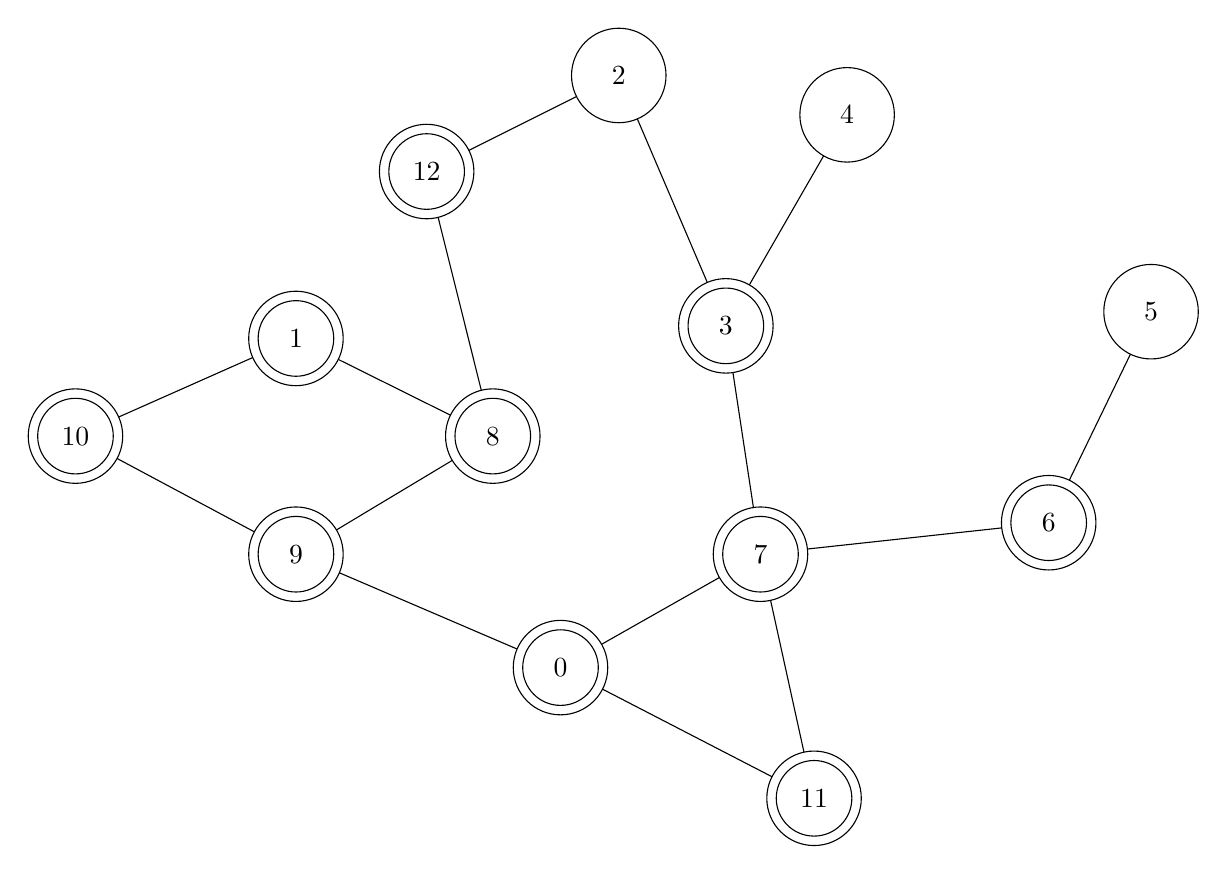
\begin{tikzpicture}[scale=0.2]
    \tikzstyle{every node}+=[inner sep=0pt]
    \draw [black] (35.4,-45.9) circle (3);
    \draw (35.4,-45.9) node {$0$};
    \draw [black] (35.4,-45.9) circle (2.4);
    \draw [black] (18.6,-38.7) circle (3);
    \draw (18.6,-38.7) node {$9$};
    \draw [black] (18.6,-38.7) circle (2.4);
    \draw [black] (51.5,-54.2) circle (3);
    \draw (51.5,-54.2) node {$11$};
    \draw [black] (51.5,-54.2) circle (2.4);
    \draw [black] (4.6,-31.2) circle (3);
    \draw (4.6,-31.2) node {$10$};
    \draw [black] (4.6,-31.2) circle (2.4);
    \draw [black] (18.6,-25) circle (3);
    \draw (18.6,-25) node {$1$};
    \draw [black] (18.6,-25) circle (2.4);
    \draw [black] (31.1,-31.2) circle (3);
    \draw (31.1,-31.2) node {$8$};
    \draw [black] (31.1,-31.2) circle (2.4);
    \draw [black] (48.1,-38.7) circle (3);
    \draw (48.1,-38.7) node {$7$};
    \draw [black] (48.1,-38.7) circle (2.4);
    \draw [black] (66.4,-36.7) circle (3);
    \draw (66.4,-36.7) node {$6$};
    \draw [black] (66.4,-36.7) circle (2.4);
    \draw [black] (45.9,-24.2) circle (3);
    \draw (45.9,-24.2) node {$3$};
    \draw [black] (45.9,-24.2) circle (2.4);
    \draw [black] (53.6,-10.8) circle (3);
    \draw (53.6,-10.8) node {$4$};
    \draw [black] (72.9,-23.3) circle (3);
    \draw (72.9,-23.3) node {$5$};
    \draw [black] (39.1,-8.3) circle (3);
    \draw (39.1,-8.3) node {$2$};
    \draw [black] (26.9,-14.4) circle (3);
    \draw (26.9,-14.4) node {$12$};
    \draw [black] (26.9,-14.4) circle (2.4);
    \draw [black] (32.64,-44.72) -- (21.36,-39.88);
    \draw [black] (38.07,-47.27) -- (48.83,-52.83);
    \draw [black] (38.01,-44.42) -- (45.49,-40.18);
    \draw [black] (48.74,-41.63) -- (50.86,-51.27);
    \draw [black] (21.17,-37.16) -- (28.53,-32.74);
    \draw [black] (15.96,-37.28) -- (7.24,-32.62);
    \draw [black] (7.34,-29.99) -- (15.86,-26.21);
    \draw [black] (28.41,-29.87) -- (21.29,-26.33);
    \draw [black] (51.08,-38.37) -- (63.42,-37.03);
    \draw [black] (47.65,-35.73) -- (46.35,-27.17);
    \draw [black] (47.39,-21.6) -- (52.11,-13.4);
    \draw [black] (67.71,-34) -- (71.59,-26);
    \draw [black] (44.72,-21.44) -- (40.28,-11.06);
    \draw [black] (30.37,-28.29) -- (27.63,-17.31);
    \draw [black] (29.58,-13.06) -- (36.42,-9.64);
    \end{tikzpicture}
\end{center}
\end{figure}

And finally repeat the same process with the next nodes

\begin{figure}[H]
\begin{center}
    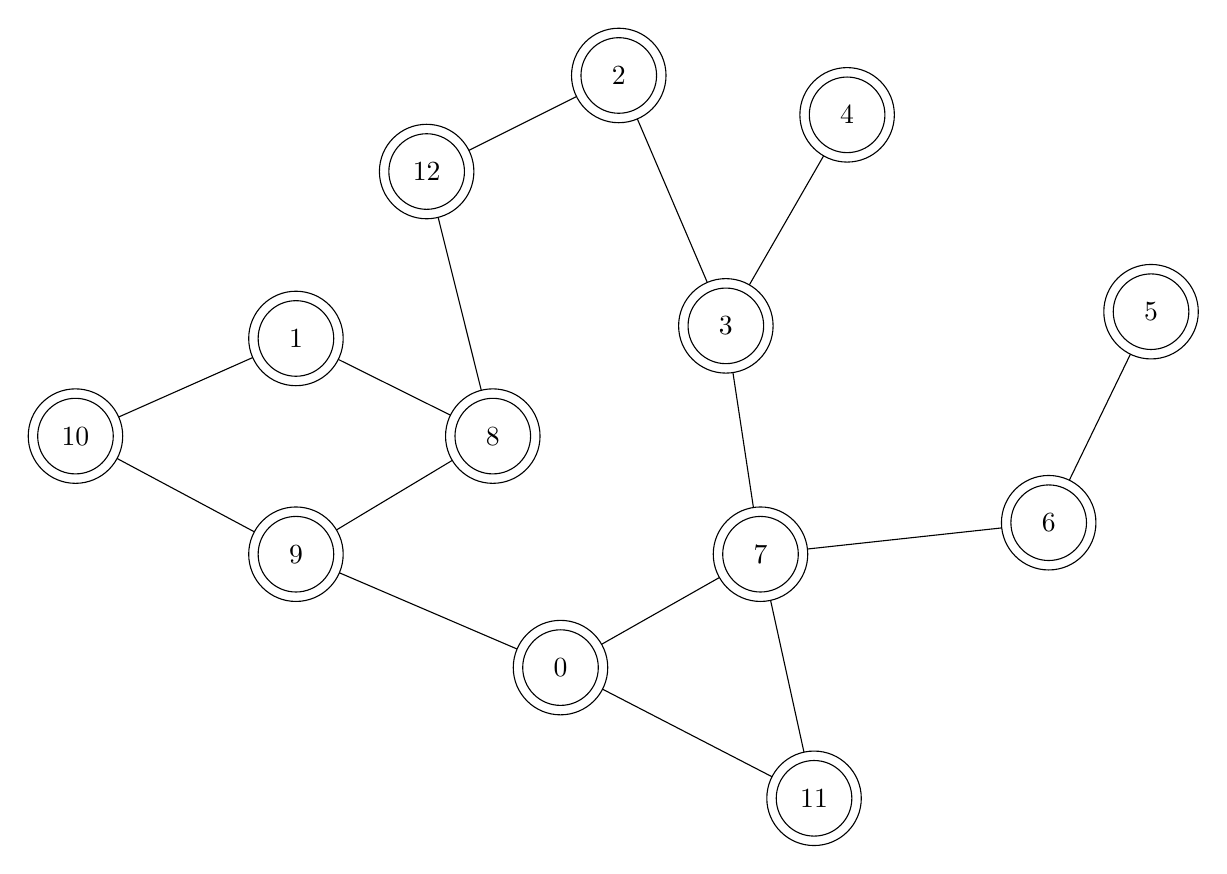
\begin{tikzpicture}[scale=0.2]
    \tikzstyle{every node}+=[inner sep=0pt]
    \draw [black] (35.4,-45.9) circle (3);
    \draw (35.4,-45.9) node {$0$};
    \draw [black] (35.4,-45.9) circle (2.4);
    \draw [black] (18.6,-38.7) circle (3);
    \draw (18.6,-38.7) node {$9$};
    \draw [black] (18.6,-38.7) circle (2.4);
    \draw [black] (51.5,-54.2) circle (3);
    \draw (51.5,-54.2) node {$11$};
    \draw [black] (51.5,-54.2) circle (2.4);
    \draw [black] (4.6,-31.2) circle (3);
    \draw (4.6,-31.2) node {$10$};
    \draw [black] (4.6,-31.2) circle (2.4);
    \draw [black] (18.6,-25) circle (3);
    \draw (18.6,-25) node {$1$};
    \draw [black] (18.6,-25) circle (2.4);
    \draw [black] (31.1,-31.2) circle (3);
    \draw (31.1,-31.2) node {$8$};
    \draw [black] (31.1,-31.2) circle (2.4);
    \draw [black] (48.1,-38.7) circle (3);
    \draw (48.1,-38.7) node {$7$};
    \draw [black] (48.1,-38.7) circle (2.4);
    \draw [black] (66.4,-36.7) circle (3);
    \draw (66.4,-36.7) node {$6$};
    \draw [black] (66.4,-36.7) circle (2.4);
    \draw [black] (45.9,-24.2) circle (3);
    \draw (45.9,-24.2) node {$3$};
    \draw [black] (45.9,-24.2) circle (2.4);
    \draw [black] (53.6,-10.8) circle (3);
    \draw (53.6,-10.8) node {$4$};
    \draw [black] (53.6,-10.8) circle (2.4);
    \draw [black] (72.9,-23.3) circle (3);
    \draw (72.9,-23.3) node {$5$};
    \draw [black] (72.9,-23.3) circle (2.4);
    \draw [black] (39.1,-8.3) circle (3);
    \draw (39.1,-8.3) node {$2$};
    \draw [black] (39.1,-8.3) circle (2.4);
    \draw [black] (26.9,-14.4) circle (3);
    \draw (26.9,-14.4) node {$12$};
    \draw [black] (26.9,-14.4) circle (2.4);
    \draw [black] (32.64,-44.72) -- (21.36,-39.88);
    \draw [black] (38.07,-47.27) -- (48.83,-52.83);
    \draw [black] (38.01,-44.42) -- (45.49,-40.18);
    \draw [black] (48.74,-41.63) -- (50.86,-51.27);
    \draw [black] (21.17,-37.16) -- (28.53,-32.74);
    \draw [black] (15.96,-37.28) -- (7.24,-32.62);
    \draw [black] (7.34,-29.99) -- (15.86,-26.21);
    \draw [black] (28.41,-29.87) -- (21.29,-26.33);
    \draw [black] (51.08,-38.37) -- (63.42,-37.03);
    \draw [black] (47.65,-35.73) -- (46.35,-27.17);
    \draw [black] (47.39,-21.6) -- (52.11,-13.4);
    \draw [black] (67.71,-34) -- (71.59,-26);
    \draw [black] (44.72,-21.44) -- (40.28,-11.06);
    \draw [black] (30.37,-28.29) -- (27.63,-17.31);
    \draw [black] (29.58,-13.06) -- (36.42,-9.64);
    \end{tikzpicture}
\end{center}
\end{figure}

Maybe understand how it works is really easy, but you need to considet that to this operation we need to use a queue. Let's see the same example but step by step.

Again we begin with the node 0.

\begin{figure}[H]
\begin{center}
    \begin{tikzpicture}[scale=0.2]
    \tikzstyle{every node}+=[inner sep=0pt]
    \draw [black] (35.4,-45.9) circle (3);
    \draw (35.4,-45.9) node {$0$};
    \draw [black] (35.4,-45.9) circle (2.4);
    \draw [black] (18.6,-38.7) circle (3);
    \draw (18.6,-38.7) node {$9$};
    \draw [black] (51.5,-54.2) circle (3);
    \draw (51.5,-54.2) node {$11$};
    \draw [black] (4.6,-31.2) circle (3);
    \draw (4.6,-31.2) node {$10$};
    \draw [black] (18.6,-25) circle (3);
    \draw (18.6,-25) node {$1$};
    \draw [black] (31.1,-31.2) circle (3);
    \draw (31.1,-31.2) node {$8$};
    \draw [black] (48.1,-38.7) circle (3);
    \draw (48.1,-38.7) node {$7$};
    \draw [black] (66.4,-36.7) circle (3);
    \draw (66.4,-36.7) node {$6$};
    \draw [black] (45.9,-24.2) circle (3);
    \draw (45.9,-24.2) node {$3$};
    \draw [black] (53.6,-10.8) circle (3);
    \draw (53.6,-10.8) node {$4$};
    \draw [black] (72.9,-23.3) circle (3);
    \draw (72.9,-23.3) node {$5$};
    \draw [black] (39.1,-8.3) circle (3);
    \draw (39.1,-8.3) node {$2$};
    \draw [black] (26.9,-14.4) circle (3);
    \draw (26.9,-14.4) node {$12$};
    \draw [black] (32.64,-44.72) -- (21.36,-39.88);
    \draw [black] (38.07,-47.27) -- (48.83,-52.83);
    \draw [black] (38.01,-44.42) -- (45.49,-40.18);
    \draw [black] (48.74,-41.63) -- (50.86,-51.27);
    \draw [black] (21.17,-37.16) -- (28.53,-32.74);
    \draw [black] (15.96,-37.28) -- (7.24,-32.62);
    \draw [black] (7.34,-29.99) -- (15.86,-26.21);
    \draw [black] (28.41,-29.87) -- (21.29,-26.33);
    \draw [black] (51.08,-38.37) -- (63.42,-37.03);
    \draw [black] (47.65,-35.73) -- (46.35,-27.17);
    \draw [black] (47.39,-21.6) -- (52.11,-13.4);
    \draw [black] (67.71,-34) -- (71.59,-26);
    \draw [black] (44.72,-21.44) -- (40.28,-11.06);
    \draw [black] (30.37,-28.29) -- (27.63,-17.31);
    \draw [black] (29.58,-13.06) -- (36.42,-9.64);
    \end{tikzpicture}
\end{center}
\end{figure}


And we add the element to our queue.

\begin{table}[H]
    \centering
    \begin{tabular}{|
    >{\columncolor[HTML]{FFFFFF}}l |}
    \hline
    {\color[HTML]{333333} } \\ \hline
                            \\ \hline
                            \\ \hline
    0                       \\ \hline
    \end{tabular}
\end{table}

Then we visit the neighbors of the current node.

\begin{figure}[H]
\begin{center}
    \begin{tikzpicture}[scale=0.2]
    \tikzstyle{every node}+=[inner sep=0pt]
    \draw [black] (35.4,-45.9) circle (3);
    \draw (35.4,-45.9) node {$0$};
    \draw [black] (35.4,-45.9) circle (2.4);
    \draw [black] (18.6,-38.7) circle (3);
    \draw (18.6,-38.7) node {$9$};
    \draw [black] (18.6,-38.7) circle (2.4);
    \draw [black] (51.5,-54.2) circle (3);
    \draw (51.5,-54.2) node {$11$};
    \draw [black] (51.5,-54.2) circle (2.4);
    \draw [black] (4.6,-31.2) circle (3);
    \draw (4.6,-31.2) node {$10$};
    \draw [black] (18.6,-25) circle (3);
    \draw (18.6,-25) node {$1$};
    \draw [black] (31.1,-31.2) circle (3);
    \draw (31.1,-31.2) node {$8$};
    \draw [black] (48.1,-38.7) circle (3);
    \draw (48.1,-38.7) node {$7$};
    \draw [black] (48.1,-38.7) circle (2.4);
    \draw [black] (66.4,-36.7) circle (3);
    \draw (66.4,-36.7) node {$6$};
    \draw [black] (45.9,-24.2) circle (3);
    \draw (45.9,-24.2) node {$3$};
    \draw [black] (53.6,-10.8) circle (3);
    \draw (53.6,-10.8) node {$4$};
    \draw [black] (72.9,-23.3) circle (3);
    \draw (72.9,-23.3) node {$5$};
    \draw [black] (39.1,-8.3) circle (3);
    \draw (39.1,-8.3) node {$2$};
    \draw [black] (26.9,-14.4) circle (3);
    \draw (26.9,-14.4) node {$12$};
    \draw [black] (32.64,-44.72) -- (21.36,-39.88);
    \draw [black] (38.07,-47.27) -- (48.83,-52.83);
    \draw [black] (38.01,-44.42) -- (45.49,-40.18);
    \draw [black] (48.74,-41.63) -- (50.86,-51.27);
    \draw [black] (21.17,-37.16) -- (28.53,-32.74);
    \draw [black] (15.96,-37.28) -- (7.24,-32.62);
    \draw [black] (7.34,-29.99) -- (15.86,-26.21);
    \draw [black] (28.41,-29.87) -- (21.29,-26.33);
    \draw [black] (51.08,-38.37) -- (63.42,-37.03);
    \draw [black] (47.65,-35.73) -- (46.35,-27.17);
    \draw [black] (47.39,-21.6) -- (52.11,-13.4);
    \draw [black] (67.71,-34) -- (71.59,-26);
    \draw [black] (44.72,-21.44) -- (40.28,-11.06);
    \draw [black] (30.37,-28.29) -- (27.63,-17.31);
    \draw [black] (29.58,-13.06) -- (36.42,-9.64);
    \end{tikzpicture}
\end{center}
\end{figure}

Also we add the elements to our queue.

\begin{table}[H]
    \centering
    \begin{tabular}{|l|}
    \rowcolor[HTML]{FFFFFF} 
    {\color[HTML]{333333} 11} \\
    \rowcolor[HTML]{FFFFFF} 
    7                         \\
    \rowcolor[HTML]{FFFFFF} 
    9                         \\
    \rowcolor[HTML]{C0C0C0} 
    0                        
    \end{tabular}
\end{table}

Now we need to visit the neighbors of the nodes 9, 7 and 11.

\begin{figure}[H]
\begin{center}
    \begin{tikzpicture}[scale=0.2]
    \tikzstyle{every node}+=[inner sep=0pt]
    \draw [black] (35.4,-45.9) circle (3);
    \draw (35.4,-45.9) node {$0$};
    \draw [black] (35.4,-45.9) circle (2.4);
    \draw [black] (18.6,-38.7) circle (3);
    \draw (18.6,-38.7) node {$9$};
    \draw [black] (18.6,-38.7) circle (2.4);
    \draw [black] (51.5,-54.2) circle (3);
    \draw (51.5,-54.2) node {$11$};
    \draw [black] (51.5,-54.2) circle (2.4);
    \draw [black] (4.6,-31.2) circle (3);
    \draw (4.6,-31.2) node {$10$};
    \draw [black] (4.6,-31.2) circle (2.4);
    \draw [black] (18.6,-25) circle (3);
    \draw (18.6,-25) node {$1$};
    \draw [black] (31.1,-31.2) circle (3);
    \draw (31.1,-31.2) node {$8$};
    \draw [black] (31.1,-31.2) circle (2.4);
    \draw [black] (48.1,-38.7) circle (3);
    \draw (48.1,-38.7) node {$7$};
    \draw [black] (48.1,-38.7) circle (2.4);
    \draw [black] (66.4,-36.7) circle (3);
    \draw (66.4,-36.7) node {$6$};
    \draw [black] (45.9,-24.2) circle (3);
    \draw (45.9,-24.2) node {$3$};
    \draw [black] (53.6,-10.8) circle (3);
    \draw (53.6,-10.8) node {$4$};
    \draw [black] (72.9,-23.3) circle (3);
    \draw (72.9,-23.3) node {$5$};
    \draw [black] (39.1,-8.3) circle (3);
    \draw (39.1,-8.3) node {$2$};
    \draw [black] (26.9,-14.4) circle (3);
    \draw (26.9,-14.4) node {$12$};
    \draw [black] (32.64,-44.72) -- (21.36,-39.88);
    \draw [black] (38.07,-47.27) -- (48.83,-52.83);
    \draw [black] (38.01,-44.42) -- (45.49,-40.18);
    \draw [black] (48.74,-41.63) -- (50.86,-51.27);
    \draw [black] (21.17,-37.16) -- (28.53,-32.74);
    \draw [black] (15.96,-37.28) -- (7.24,-32.62);
    \draw [black] (7.34,-29.99) -- (15.86,-26.21);
    \draw [black] (28.41,-29.87) -- (21.29,-26.33);
    \draw [black] (51.08,-38.37) -- (63.42,-37.03);
    \draw [black] (47.65,-35.73) -- (46.35,-27.17);
    \draw [black] (47.39,-21.6) -- (52.11,-13.4);
    \draw [black] (67.71,-34) -- (71.59,-26);
    \draw [black] (44.72,-21.44) -- (40.28,-11.06);
    \draw [black] (30.37,-28.29) -- (27.63,-17.31);
    \draw [black] (29.58,-13.06) -- (36.42,-9.64);
    \end{tikzpicture}
\end{center}
\end{figure}

We add the nodes to our queue.

\begin{table}[H]
    \centering
    \begin{tabular}{|l|}
    \hline
                              \\ \hline
    8                         \\ \hline
    10                        \\ \hline
    \rowcolor[HTML]{FFFFFF} 
    {\color[HTML]{333333} 11} \\ \hline
    \rowcolor[HTML]{FFFFFF} 
    7                         \\ \hline
    \rowcolor[HTML]{EFEFEF} 
    9                         \\ \hline
    \rowcolor[HTML]{EFEFEF} 
    0                         \\ \hline
    \end{tabular}
\end{table}

We continue doing the same until we have all the nodes in the queue.

\begin{figure}[H]
\begin{center}
    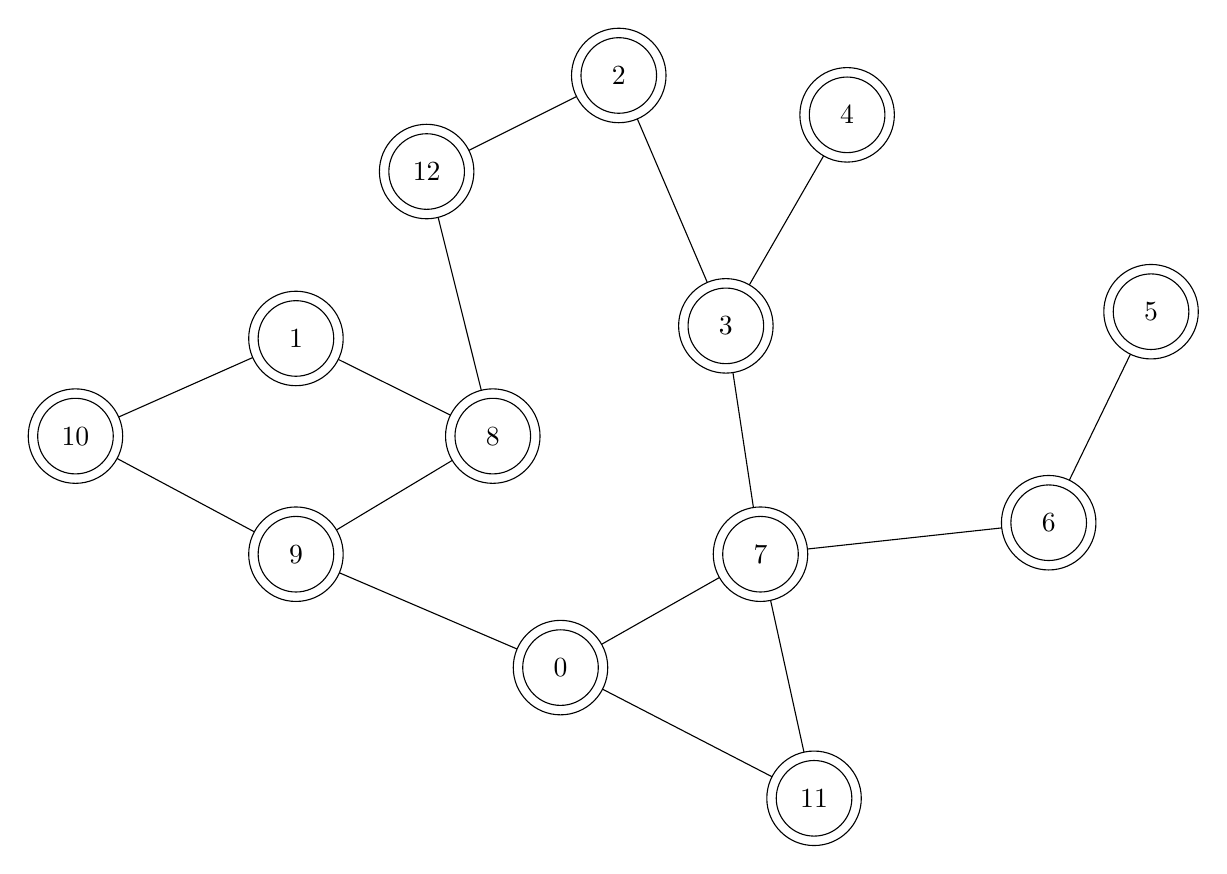
\begin{tikzpicture}[scale=0.2]
    \tikzstyle{every node}+=[inner sep=0pt]
    \draw [black] (35.4,-45.9) circle (3);
    \draw (35.4,-45.9) node {$0$};
    \draw [black] (35.4,-45.9) circle (2.4);
    \draw [black] (18.6,-38.7) circle (3);
    \draw (18.6,-38.7) node {$9$};
    \draw [black] (18.6,-38.7) circle (2.4);
    \draw [black] (51.5,-54.2) circle (3);
    \draw (51.5,-54.2) node {$11$};
    \draw [black] (51.5,-54.2) circle (2.4);
    \draw [black] (4.6,-31.2) circle (3);
    \draw (4.6,-31.2) node {$10$};
    \draw [black] (4.6,-31.2) circle (2.4);
    \draw [black] (18.6,-25) circle (3);
    \draw (18.6,-25) node {$1$};
    \draw [black] (18.6,-25) circle (2.4);
    \draw [black] (31.1,-31.2) circle (3);
    \draw (31.1,-31.2) node {$8$};
    \draw [black] (31.1,-31.2) circle (2.4);
    \draw [black] (48.1,-38.7) circle (3);
    \draw (48.1,-38.7) node {$7$};
    \draw [black] (48.1,-38.7) circle (2.4);
    \draw [black] (66.4,-36.7) circle (3);
    \draw (66.4,-36.7) node {$6$};
    \draw [black] (66.4,-36.7) circle (2.4);
    \draw [black] (45.9,-24.2) circle (3);
    \draw (45.9,-24.2) node {$3$};
    \draw [black] (45.9,-24.2) circle (2.4);
    \draw [black] (53.6,-10.8) circle (3);
    \draw (53.6,-10.8) node {$4$};
    \draw [black] (53.6,-10.8) circle (2.4);
    \draw [black] (72.9,-23.3) circle (3);
    \draw (72.9,-23.3) node {$5$};
    \draw [black] (72.9,-23.3) circle (2.4);
    \draw [black] (39.1,-8.3) circle (3);
    \draw (39.1,-8.3) node {$2$};
    \draw [black] (39.1,-8.3) circle (2.4);
    \draw [black] (26.9,-14.4) circle (3);
    \draw (26.9,-14.4) node {$12$};
    \draw [black] (26.9,-14.4) circle (2.4);
    \draw [black] (32.64,-44.72) -- (21.36,-39.88);
    \draw [black] (38.07,-47.27) -- (48.83,-52.83);
    \draw [black] (38.01,-44.42) -- (45.49,-40.18);
    \draw [black] (48.74,-41.63) -- (50.86,-51.27);
    \draw [black] (21.17,-37.16) -- (28.53,-32.74);
    \draw [black] (15.96,-37.28) -- (7.24,-32.62);
    \draw [black] (7.34,-29.99) -- (15.86,-26.21);
    \draw [black] (28.41,-29.87) -- (21.29,-26.33);
    \draw [black] (51.08,-38.37) -- (63.42,-37.03);
    \draw [black] (47.65,-35.73) -- (46.35,-27.17);
    \draw [black] (47.39,-21.6) -- (52.11,-13.4);
    \draw [black] (67.71,-34) -- (71.59,-26);
    \draw [black] (44.72,-21.44) -- (40.28,-11.06);
    \draw [black] (30.37,-28.29) -- (27.63,-17.31);
    \draw [black] (29.58,-13.06) -- (36.42,-9.64);
    \end{tikzpicture}
\end{center}
\end{figure}

\begin{table}[H]
    \centering
    \begin{tabular}{|l|}
    \hline
    4                         \\ \hline
    2                         \\ \hline
    5                         \\ \hline
    12                        \\ \hline
    1                         \\ \hline
    \rowcolor[HTML]{EFEFEF} 
    3                         \\ \hline
    \rowcolor[HTML]{EFEFEF} 
    6                         \\ \hline
    \rowcolor[HTML]{EFEFEF} 
    8                         \\ \hline
    \rowcolor[HTML]{EFEFEF} 
    10                        \\ \hline
    \rowcolor[HTML]{EFEFEF} 
    {\color[HTML]{333333} 11} \\ \hline
    \rowcolor[HTML]{EFEFEF} 
    7                         \\ \hline
    \rowcolor[HTML]{EFEFEF} 
    9                         \\ \hline
    \rowcolor[HTML]{EFEFEF} 
    0                         \\ \hline
    \end{tabular}
\end{table}

Finally we need to continue doing the same process until the queue is empty.\\\\

\subsubsection{Using a queue}
The BFS algorithm uses a queue data structure to track which node to visit next. Upon reaching a new node the algorithm adds it to the queue to visit it later. The queue data structure works just like a real world queue such a waiting line at a restaurant. People can either enter the waiting line (enqueue) or get seated (dequeue).

Here you are the code to the function to make the Breath First Search. Consider the same structure for a graph that I implemented in the DFS section.

\begin{lstlisting}
    void BFS( lli u ){
        queue< lli > Queue;
        Queue.push( u );

        while( !Queue.empty() ){
            u = Queue.front();
            Queue.pop();
            nodes[ u ].visited = true;
            nodes[ u ].value = 1;

            for( int i = 0; i < nodes[ u ].adjList.size(); i++ ){
                lli v = nodes[ u ].adjList[ i ];
                if( !nodes[ v ].visited )
                    Queue.push( v );
            }
        }
    }
\end{lstlisting}

\subsubsection{Shortest path in an unweighted graph}

